\section{Decision-Theoretic Planning}

\begin{frame}
\frametitle{Decision-Theoretic Planning}
\framesubtitle{DTP Problem Scope}

\begin{columns}[T]
 	\begin{column}{.7\textwidth}
	\textbf{Systems:}
	\begin{itemize}
		\item Dynamics are stochastic, i.e., involve uncertainty
		\begin{itemize}
			\item Execution of actions (e.g., robot may slip)
			\item Exogenous events (e.g., doors open/closed)
			\item Observations (e.g., sensor noise)
		\end{itemize}
		\item Controlled by one or more agents
		\item Sequential decisions of actions to execute
	\end{itemize}
%	\textbf{Examples:}
%	\begin{itemize}
%		\item Motion Planning
%		\item Path Planning
%	\end{itemize}
 	\end{column}
 	\begin{column}{.35\textwidth}
 		%\vspace{-30pt}
 		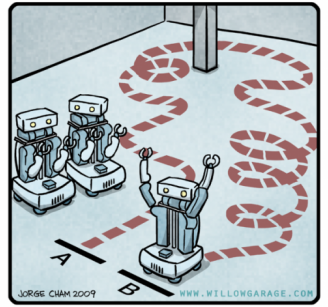
\includegraphics[width=1.0\textwidth, right]{figures/path-planning2}
 	\end{column}
\end{columns}

\end{frame}

\begin{frame}
\frametitle{Decision-Theoretic Planning}
\framesubtitle{Example Domain: Path Planning}
\centering

\begin{columns}[T]
	\begin{column}{.6\textwidth}
		\centering
	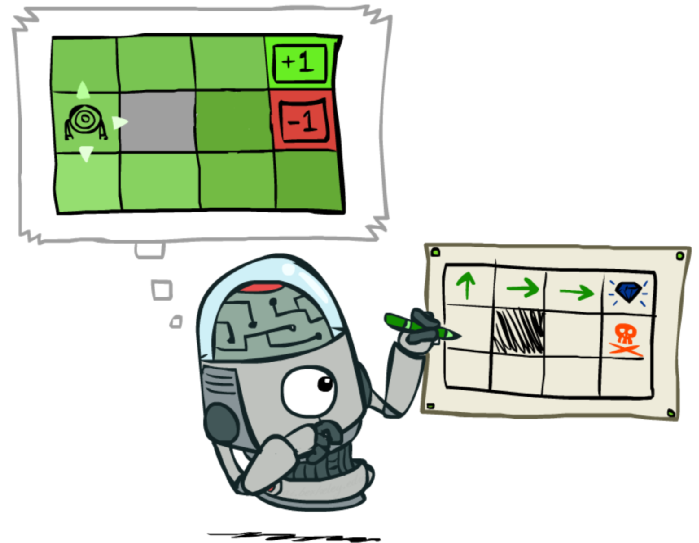
\includegraphics[width=0.7\textwidth]{figures/path-planning3}
	\vfill
	{\tiny Source: \href{http://ai.berkeley.edu/lecture_slides.html}{Berkeley CS188 sheets}}
	\end{column}
	\begin{column}{.5\textwidth}
		\centering
		\vspace{20pt}
		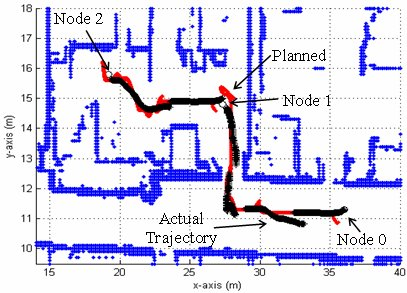
\includegraphics[width=0.75\textwidth]{figures/path-planning4}\\
		\vspace{2.5pt}
		{\tiny Source: \url{http://www.cs.cmu.edu/~gunhee/r\_psr.html}}
	\end{column}
\end{columns}

\end{frame}

\begin{frame}
\frametitle{Decision-Theoretic Planning}
\framesubtitle{Example Domain: Motion Planning}
\begin{center}
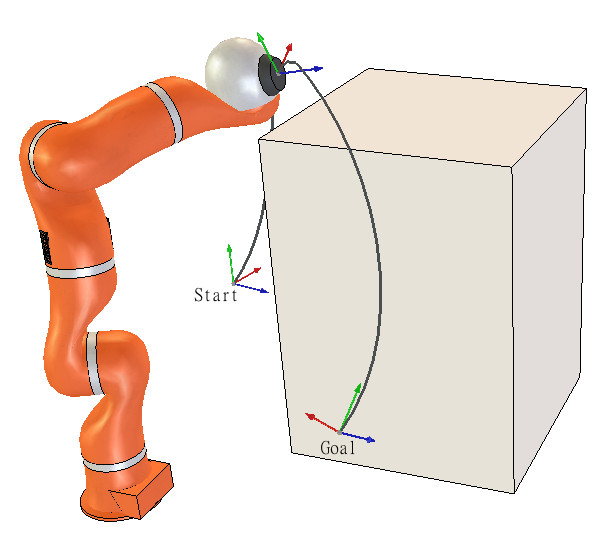
\includegraphics[width=0.38\textwidth]{figures/motion-planning}
\vfill
{\tiny Source: \url{http://www.coppeliarobotics.com/helpFiles/en/motionPlanningModule.htm}}
\end{center}
\end{frame}

\begin{frame}
\frametitle{Decision-Theoretic Planning}
\framesubtitle{Markov Decision Processes (MDPs)}

In DTP systems are modeled by probabilistic models, e.g. MDPs:
\begin{columns}[T]
\begin{column}{0.65\textwidth}
	\begin{definition}
	An MDP is a 5-tuple $\mathcal{M} = (\mathcal{S}, s_0, A, \delta, R)$:
	\begin{itemize}
		\item $\mathcal{S}$ is the state-space, $s_0 \in \mathcal{S}$ the initial state
		\item $A$ is the action-space
		\item $\delta$ is the transition function (N.B.: accounts for uncertainty) % $\delta: S \times S \times A \mapsto [0,1]$
		\item $R$ is the reward function (N.B.: defines the goals)
	\end{itemize}
	\end{definition}
\end{column}

\begin{column}{0.375\textwidth}
	\vspace{32pt}
%	\begin{tikzpicture}[->,>=stealth',auto,node distance=2cm]
%	\tikzstyle{every state}=[fill=white,draw=black,text=black,scale=1, thick]	% thick
%	\node[state] (s1) {$q_t$};
%	\node[state] (s2) [right of=s1] {$q_{t+1}$};
%	\path
%	(s1)
%	edge node {} (s2)
%	(s2);
%	;
%	\end{tikzpicture}
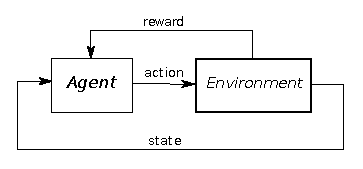
\includegraphics{figures/mdp}
\end{column}
\end{columns}
\end{frame}

\begin{frame}
\frametitle{Decision-Theoretic Planning}
\framesubtitle{Learning Optimal Plans}

\begin{center}
	\vspace{-12pt}
	\includegraphics<1| handout:0>[width=0.95\textwidth]{figures/planning-routine/mdp-planning-diagram-v2-1.pdf}
	\includegraphics<2|handout:0>[width=0.95\textwidth]{figures/planning-routine/mdp-planning-diagram-v2-2.pdf}
	\includegraphics<3|handout:0>[width=0.95\textwidth]{figures/planning-routine/mdp-planning-diagram-v2-3.pdf}
	\includegraphics<4|handout:0>[width=0.95\textwidth]{figures/planning-routine/mdp-planning-diagram-v2-4.pdf}
	\includegraphics<5>[width=0.95\textwidth]{figures/planning-routine/mdp-planning-diagram-v2-5.pdf}
\end{center}

\end{frame}

\begin{frame}
\frametitle{Decision-Theoretic Planning}
\framesubtitle{Model Development}

%\begin{center}
	\textcolor{tudBlack}{\textbf{Problem:}} How to find a suitable MDP model?
	\pause
	\vfill
	\textcolor{tudBlack}{\textbf{Classical approach:}} Model development by a \textit{human designer}, however:
	\begin{itemize}
		\item Requires significant effort (e.g., trial-and-error)
		\item Typically demands knowledge/experience, accompanied by high costs
	\end{itemize}
	\pause
	\vfill
	\textcolor{tudBlack}{\textbf{Alternative:}} Use Reinforcement Learning instead of Planning, however:
	\begin{itemize}
		\item Requires direct interaction with environment %(slow in complex dynamic environment) % (chance of errors)
		\item One might require \textit{reusable} models, applicable for multiple tasks % You do have model-based RL, but we might want a model that generalizes for multiple tasks
		%\item Still requires definition of state-spaces (and actions and rewards)
	\end{itemize}

%\end{center}
\end{frame}

\begin{frame}[t]
\frametitle{Decision-Theoretic Planning}
\framesubtitle{Model Development}
\vspace{8pt}
\textcolor{tudBlack}{\textbf{Problem:}} How to find a suitable MDP model?\\
\vspace{14pt}
\textcolor{tudblue}{\textbf{Idea:}} Automate the model building process by learning algorithms 
\begin{itemize}
	\item Learn from (exploration) data about the environment
	\item Optimization for the best MDP model
\end{itemize}

\end{frame}